
\documentclass[aspectratio=169,11pt]{beamer}

\usetheme{Boadilla}
\usecolortheme{seahorse}
\setbeamertemplate{navigation symbols}{}
\setbeamertemplate{caption}[numbered]
\setbeamertemplate{footline}[frame number]

\usepackage{fontspec}
\setsansfont{Latin Modern Sans}
\usepackage[spanish,es-tabla]{babel}
\usepackage{graphicx}
\usepackage{booktabs}
\usepackage{tikz}
\usepackage{listings}
\usepackage{xcolor}
\usepackage{array}
\usepackage{hyperref}

\hypersetup{
  colorlinks=true,
  urlcolor=perkblue,
  linkcolor=perkblue
}
\usetikzlibrary{arrows.meta,positioning,shapes.geometric,fit,calc}

\definecolor{perkblue}{HTML}{2D6CDF}
\definecolor{perkcyan}{HTML}{19A7CE}
\definecolor{perkorange}{HTML}{F28C28}
\definecolor{perkgray}{HTML}{5B6470}
\definecolor{perkbg}{HTML}{F7F9FC}
\definecolor{perkgreen}{HTML}{4CAF50}

\setbeamercolor{title}{fg=perkblue}
\setbeamercolor{frametitle}{fg=perkblue}
\setbeamercolor{structure}{fg=perkblue}
\setbeamercolor{block title}{bg=perkblue, fg=white}
\setbeamercolor{block body}{bg=perkbg, fg=black}

\lstdefinestyle{perkcode}{
  basicstyle=\ttfamily\scriptsize,
  backgroundcolor=\color{perkbg},
  frame=single,
  rulecolor=\color{perkgray!35},
  breaklines=true,
  columns=fullflexible,
  keepspaces=true
}
\lstset{style=perkcode}

\newcommand{\pill}[1]{\tikz[baseline=(x.base)]\node[rounded corners=3pt, fill=perkblue!10, draw=perkblue!30, inner xsep=5pt, inner ysep=2pt](x){\scriptsize #1};}
\newcommand{\codefile}[1]{\texttt{#1}}

\title[PERK-ID]{PERK-ID: búsqueda visual de pastillas}
\author{Bioinformática y Medicina}
\institute{Grado en Inteligencia Artificial}
\date{}

\begin{document}

% 1
\begin{frame}
  \titlepage
  \begin{center}
    \vspace{-0.4cm}
    %\includegraphics[height=2.0cm]{logo.jpeg}
  \end{center}

\end{frame}

% 2
\begin{frame}{Problema que resuelve}
  \centering

  \vfill

  \begin{columns}[c,onlytextwidth]

    \column{0.50\textwidth}
      \begin{block}{Objetivo principal}
      Recuperar, a partir de una foto de entrada, las pastillas del dataset que más se parecen visualmente.
      \end{block}

      \vspace{0.25cm}

      \begin{itemize}
        \item Entrada: imagen desde cámara o galería.
        \item Salida: ranking Top-K con imagen, metadatos y sustancias asociadas.
        \item Enfoque: recuperación de imágenes por similitud.
      \end{itemize}

    \column{0.42\textwidth}
      \centering
      \begin{tikzpicture}[
        node distance=0.45cm,
        box/.style={
          draw,
          rounded corners=6pt,
          minimum width=3.8cm,
          minimum height=0.78cm,
          align=center,
          font=\small,
          thick
        },
        arrow/.style={
          -{Latex[length=2.5mm]},
          thick,
          perkblue
        }
      ]

      \node[box, fill=perkcyan!15, draw=perkcyan] (foto) {
        \textbf{Foto}\\
        cámara o galería
      };

      \node[box, fill=perkorange!15, draw=perkorange, below=of foto] (features) {
        \textbf{Descriptores}\\
        forma, textura, marcas
      };

      \node[box, fill=perkgreen!15, draw=perkgreen, below=of features] (busqueda) {
        \textbf{Búsqueda}\\
        imágenes similares
      };

      \node[box, fill=perkblue!10, draw=perkblue, below=of busqueda] (ranking) {
        \textbf{Resultado}\\
        Top-K pastillas
      };

      \draw[arrow] (foto) -- (features);
      \draw[arrow] (features) -- (busqueda);
      \draw[arrow] (busqueda) -- (ranking);

      \end{tikzpicture}

  \end{columns}

  \vfill
\end{frame}



% 3
\begin{frame}{Dataset}
  \begin{columns}[T,onlytextwidth]

    % IZQUIERDA
    \column{0.46\textwidth}

      {\footnotesize
      \begin{block}{Datos de partida}
      Imágenes y metadatos de pastillas obtenidos mediante extracción automatizada, procedentes de\\ \href{https://energycontrol.org/}{Energy Control}.
      \end{block}

      \vspace{0.1cm}

      \begin{itemize}
        \setlength\itemsep{0.06cm}
        \item Cada registro corresponde a una pastilla analizada.
        \item Se guardan imágenes cuando están disponibles.
        \item Los metadatos incluyen color, logo, procedencia, peso, diámetro y sustancias.
        \item La información queda estructurada en una tabla junto con las rutas de imagen.
        \item Antes de compararlas, las imágenes se normalizan: RGB, recorte centrado y tamaño fijo.
      \end{itemize}
      }

    % DERECHA
    \column{0.50\textwidth}
      \centering

      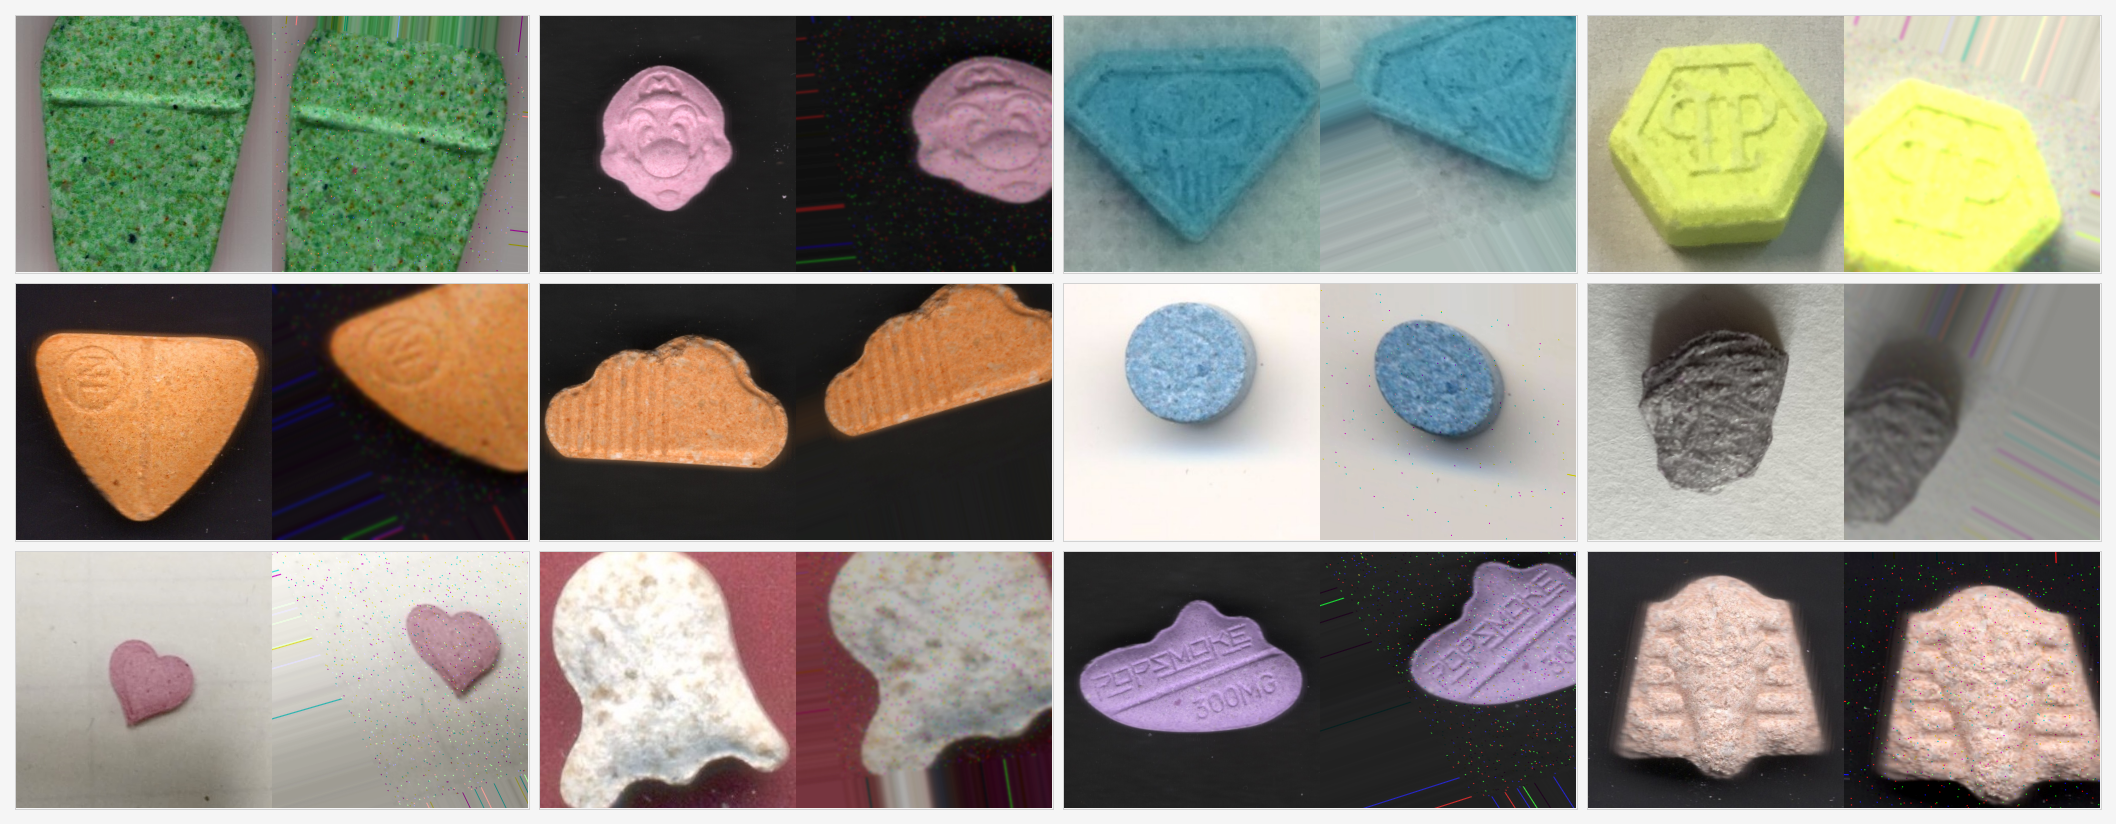
\includegraphics[width=\linewidth]{imagenes/transform_grid.png}

      \vspace{0.1cm}

      {\scriptsize Ejemplos de transformaciones para simular capturas reales.}

      \vspace{0.22cm}

      \begin{tikzpicture}[
        node distance=0.28cm,
        box/.style={
          draw,
          rounded corners=5pt,
          minimum width=4.1cm,
          minimum height=0.42cm,
          align=center,
          font=\scriptsize,
          thick
        },
        arrow/.style={
          -{Latex[length=1.8mm]},
          thick,
          perkblue
        }
      ]

      \node[box, fill=perkcyan!15, draw=perkcyan] (source) {Energy Control};
      \node[box, fill=perkorange!15, draw=perkorange, below=of source] (extract) {Extracción automatizada};
      \node[box, fill=perkblue!10, draw=perkblue, below=of extract] (table) {Tabla de metadatos};
      \node[box, fill=perkgreen!15, draw=perkgreen, below=of table] (images) {Imágenes normalizadas};

      \draw[arrow] (source) -- (extract);
      \draw[arrow] (extract) -- (table);
      \draw[arrow] (table) -- (images);

      \end{tikzpicture}

  \end{columns}
\end{frame}


% 4

\begin{frame}{Arquitectura general}
  \centering

  \vfill

  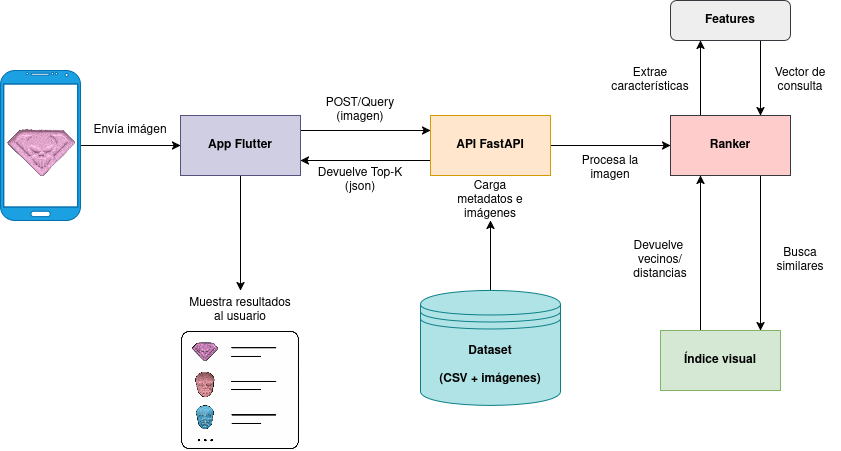
\includegraphics[width=0.95\linewidth]{imagenes/arquitectura_app.png}

  \vfill

  \pill{Frontend} \hspace{0.4cm}
  \pill{API} \hspace{0.4cm}
  \pill{Ranking visual} \hspace{0.4cm}
  \pill{Datos}

\end{frame}

% 6
\begin{frame}{Preprocesado}
  \begin{columns}[c,onlytextwidth]

    \column{0.44\textwidth}

      \begin{block}{Normalización}
      Todas las imágenes se llevan al mismo formato antes de calcular los descriptores visuales.
      \end{block}

      \vspace{0.15cm}

      \begin{itemize}
        \setlength\itemsep{0.18cm}
        \item Conversión a RGB.
        \item Recorte centrado.
        \item Redimensionado a \(256 \times 256\).
        \item Salida homogénea para comparar imágenes.
      \end{itemize}

      \vspace{0.2cm}

      {\footnotesize
      Esto evita que el ranking dependa de diferencias de escala, formato o encuadre.
      }

    \column{0.52\textwidth}
      \centering

      \begin{tikzpicture}[
        node distance=0.50cm,
        box/.style={
          draw,
          rounded corners=5pt,
          minimum width=4.7cm,
          minimum height=0.62cm,
          align=center,
          font=\small,
          thick
        },
        arrow/.style={
          -{Latex[length=2mm]},
          thick,
          perkblue
        }
      ]

      \node[box, fill=perkcyan!15, draw=perkcyan] (input) {Imagen original};
      \node[box, fill=perkorange!15, draw=perkorange, below=of input] (rgb) {Conversión a RGB};
      \node[box, fill=perkblue!10, draw=perkblue, below=of rgb] (crop) {Recorte centrado};
      \node[box, fill=perkgreen!15, draw=perkgreen, below=of crop] (resize) {Resize \(256 \times 256\)};
      \node[box, fill=perkgray!10, draw=perkgray, below=of resize] (output) {Imagen normalizada};

      \draw[arrow] (input) -- (rgb);
      \draw[arrow] (rgb) -- (crop);
      \draw[arrow] (crop) -- (resize);
      \draw[arrow] (resize) -- (output);

      \end{tikzpicture}

  \end{columns}
\end{frame}


% 7
\begin{frame}{Descriptores visuales utilizados}
  \begin{columns}[c,onlytextwidth]

    \column{0.48\textwidth}
      \centering

      \begin{tikzpicture}[
        node distance=0.38cm,
        box/.style={
          draw,
          rounded corners=5pt,
          minimum width=4.2cm,
          minimum height=0.58cm,
          align=center,
          font=\scriptsize,
          thick
        },
        arrow/.style={
          -{Latex[length=2mm]},
          thick,
          perkblue
        }
      ]

      \node[box, fill=perkcyan!15, draw=perkcyan] (img) {
        Imagen normalizada
      };

      \node[box, fill=perkorange!15, draw=perkorange, below=of img] (sift) {
        SIFT: puntos locales
      };

      \node[box, fill=perkorange!10, draw=perkorange, below=of sift] (bow) {
        BoW: histograma visual
      };

      \node[box, fill=perkblue!10, draw=perkblue, below=of bow] (classic) {
        GLCM + Hu Moments + LBP
      };

      \node[box, fill=perkgreen!15, draw=perkgreen, below=of classic] (vector) {
        Vector final de características
      };

      \draw[arrow] (img) -- (sift);
      \draw[arrow] (sift) -- (bow);
      \draw[arrow] (bow) -- (classic);
      \draw[arrow] (classic) -- (vector);

      \end{tikzpicture}

      \vspace{0.25cm}

      {\scriptsize Todos los descriptores se concatenan para representar cada pastilla mediante un vector comparable.}

    \column{0.48\textwidth}

      \begin{itemize}
        \setlength\itemsep{0.18cm}
        \item \textbf{SIFT}: detecta puntos locales, logos, letras y bordes.
        \item \textbf{BoW}: convierte los descriptores SIFT en un vector fijo.
        \item \textbf{GLCM}: describe la textura global en escala de grises.
        \item \textbf{Hu Moments}: resume la forma global de la pastilla.
        \item \textbf{LBP}: captura microtexturas y patrones locales.
      \end{itemize}

  \end{columns}
\end{frame}


% 8
\begin{frame}{Cómo se construye el índice}
  \begin{columns}[T,onlytextwidth]
    \column{0.48\textwidth}
      \begin{enumerate}
        \item Leer cada imagen del dataset.
        \item Extraer GLCM, Hu Moments y LBP.
        \item Extraer descriptores SIFT.
        \item Entrenar KMeans para Bag of Words.
        \item Concatenar todo en un vector final.
        \item Guardar matriz de features e imágenes asociadas.
      \end{enumerate}
    \column{0.48\textwidth}
      \begin{tikzpicture}[node distance=0.45cm]
        \node[draw, rounded corners, fill=perkcyan!15, minimum width=4.8cm, minimum height=0.7cm] (img) {Imagen};
        \node[draw, rounded corners, fill=perkblue!10, below=of img, minimum width=4.8cm, minimum height=0.7cm] (desc) {Descriptores clásicos};
        \node[draw, rounded corners, fill=perkorange!15, below=of desc, minimum width=4.8cm, minimum height=0.7cm] (sift) {SIFT → BoW};
        \node[draw, rounded corners, fill=perkgreen!15, below=of sift, minimum width=4.8cm, minimum height=0.7cm] (vec) {Vector final};
        \node[draw, rounded corners, fill=perkgray!10, below=of vec, minimum width=4.8cm, minimum height=0.7cm] (npz) {\codefile{features.npz}};
        \draw[-{Latex[length=3mm]}, thick] (img) -- (desc);
        \draw[-{Latex[length=3mm]}, thick] (desc) -- (sift);
        \draw[-{Latex[length=3mm]}, thick] (sift) -- (vec);
        \draw[-{Latex[length=3mm]}, thick] (vec) -- (npz);
      \end{tikzpicture}
  \end{columns}

\end{frame}

% 9
\begin{frame}{Consulta y ranking}
  \begin{columns}[c,onlytextwidth]

    \column{0.54\textwidth}
      \begin{block}{Funcionamiento}
      A partir de una imagen de consulta, el sistema extrae sus descriptores visuales y busca en el índice las pastillas más parecidas.
      \end{block}

      \vspace{0.2cm}

      \begin{itemize}
        \setlength\itemsep{0.16cm}
        \item Se calcula un vector de características para la imagen de entrada.
        \item Ese vector se compara con los vectores del índice visual.
        \item La búsqueda se realiza mediante vecinos más cercanos.
        \item Como resultado, se obtiene un ranking ordenado por similitud.
      \end{itemize}

    \column{0.42\textwidth}
      \centering

      \begin{tikzpicture}[
        node distance=0.38cm,
        box/.style={
          draw,
          rounded corners=5pt,
          minimum width=4.1cm,
          minimum height=0.58cm,
          align=center,
          font=\scriptsize,
          thick
        },
        arrow/.style={
          -{Latex[length=2mm]},
          thick,
          perkblue
        }
      ]

      \node[box, fill=perkcyan!15, draw=perkcyan] (query) {Imagen de consulta};
      \node[box, fill=perkorange!15, draw=perkorange, below=of query] (desc) {Extracción de descriptores};
      \node[box, fill=perkblue!10, draw=perkblue, below=of desc] (index) {Comparación con el índice};
      \node[box, fill=perkgreen!15, draw=perkgreen, below=of index] (rank) {Ranking Top-K};

      \draw[arrow] (query) -- (desc);
      \draw[arrow] (desc) -- (index);
      \draw[arrow] (index) -- (rank);

      \end{tikzpicture}

      \vspace{0.25cm}

      \begin{block}{Interpretación}
      Cuanto menor es la distancia, mayor es la similitud visual con la imagen de entrada.
      \end{block}

  \end{columns}
\end{frame}

% 10
\begin{frame}{Backend FastAPI}
  \begin{columns}[c,onlytextwidth]

    \column{0.54\textwidth}
      \begin{block}{Funcionamiento}
      El backend actúa como intermediario entre la app y el sistema de búsqueda visual: recibe la imagen, consulta el ranking y construye la respuesta final.
      \end{block}

      \vspace{0.2cm}

      \begin{itemize}
        \setlength\itemsep{0.16cm}
        \item Recibe la imagen enviada desde la app mediante una petición \texttt{POST /query}.
        \item Carga el índice visual y los metadatos necesarios para resolver la consulta.
        \item Llama al módulo de ranking para obtener las pastillas más similares.
        \item Devuelve una respuesta estructurada con resultados, metadatos y sustancias asociadas.
      \end{itemize}

    \column{0.42\textwidth}
      \centering

      \begin{tikzpicture}[
        node distance=0.38cm,
        box/.style={
          draw,
          rounded corners=5pt,
          minimum width=4.1cm,
          minimum height=0.58cm,
          align=center,
          font=\scriptsize,
          thick
        },
        arrow/.style={
          -{Latex[length=2mm]},
          thick,
          perkblue
        }
      ]

      \node[box, fill=perkcyan!15, draw=perkcyan] (request) {Petición desde Flutter};
      \node[box, fill=perkorange!15, draw=perkorange, below=of request] (api) {Procesamiento en FastAPI};
      \node[box, fill=perkblue!10, draw=perkblue, below=of api] (rank) {Consulta al ranking};
      \node[box, fill=perkgreen!15, draw=perkgreen, below=of rank] (json) {Respuesta JSON Top-K};

      \draw[arrow] (request) -- (api);
      \draw[arrow] (api) -- (rank);
      \draw[arrow] (rank) -- (json);

      \end{tikzpicture}

      \vspace{0.25cm}

      \begin{block}{Respuesta}
      La app recibe un JSON con las imágenes candidatas, sus distancias de similitud y los metadatos asociados.
      \end{block}

  \end{columns}
\end{frame}

% 11
\begin{frame}{Frontend Flutter}
  \begin{columns}[c,onlytextwidth]

    \column{0.52\textwidth}

      \begin{block}{Papel de la app}
      La app actúa como interfaz entre el usuario y el backend: captura la imagen, lanza la consulta y muestra los resultados.
      \end{block}

      \vspace{0.25cm}

      \begin{itemize}
        \setlength\itemsep{0.18cm}
        \item Permite usar la cámara o seleccionar una imagen de la galería.
        \item Envía la imagen al backend mediante una petición HTTP.
        \item Permite elegir cuántos resultados mostrar.
        \item Presenta el ranking de pastillas similares en tarjetas.
      \end{itemize}

    \column{0.44\textwidth}

      \begin{block}{Tecnologías utilizadas}
      \begin{itemize}
        \setlength\itemsep{0.16cm}
        \item \textbf{Flutter}: framework para construir la app móvil/web.
        \item \textbf{Dart}: lenguaje usado por Flutter.
        \item \textbf{camera}: acceso a la cámara del dispositivo.
        \item \textbf{image\_picker}: selección de imágenes desde galería.
        \item \textbf{http}: envío de peticiones al backend.
        \item \textbf{shared\_preferences}: guardado de configuración local.
      \end{itemize}
      \end{block}

  \end{columns}
\end{frame}


% 12
\begin{frame}{Evaluación del índice}
  \begin{columns}[c,onlytextwidth]

    \column{0.44\textwidth}

      \begin{block}{Objetivo}
      Evaluar si el índice recupera la pastilla original cuando la consulta es una versión transformada.
      \end{block}

      \vspace{0.12cm}

      \begin{block}{Proceso}
      \begin{itemize}
        \setlength\itemsep{0.03cm}
        \item Se toman imágenes ya indexadas.
        \item Se generan consultas transformadas.
        \item Se compara cada consulta contra el índice.
        \item Se registra la posición de la imagen original.
      \end{itemize}
      \end{block}

      \vspace{0.03cm}

      {\scriptsize
      \textbf{Métricas:} Top-1, Top-K, ranking medio, distancia media y tiempo de consulta.
      }

    \column{0.52\textwidth}
      \centering

      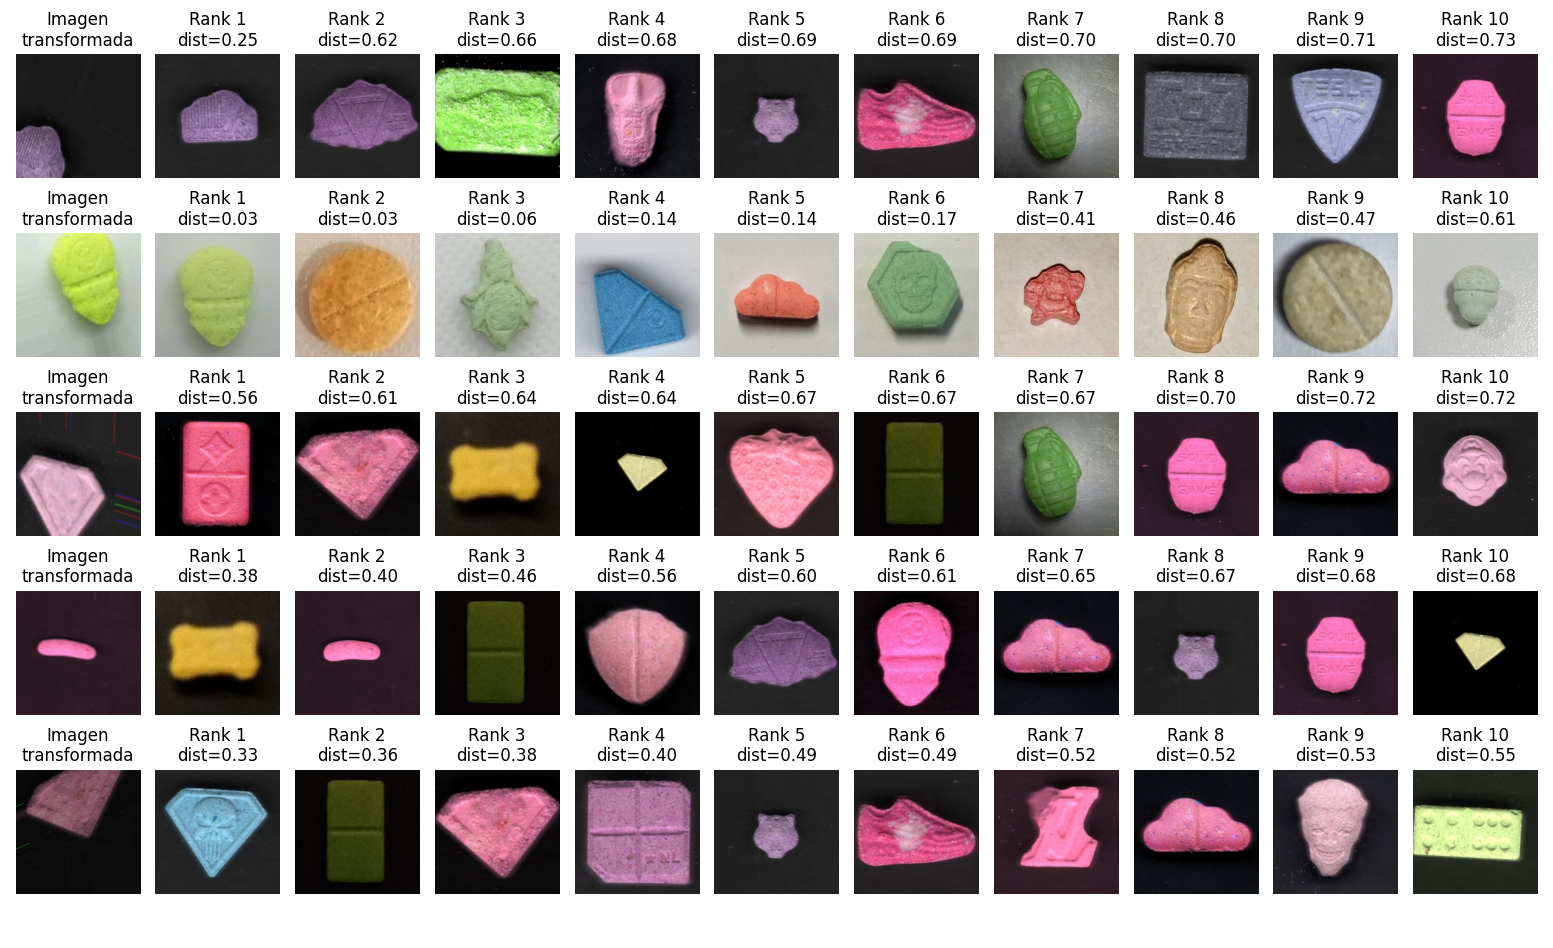
\includegraphics[width=\linewidth]{imagenes/eval.png}

      \vspace{0.12cm}

      {\scriptsize Ejemplo visual: cada fila muestra una consulta transformada y los resultados recuperados por el índice.}

  \end{columns}
\end{frame}


% 13
\begin{frame}{Módulo experimental: autoencoder y bounding boxes}

\end{frame}

% 14
\begin{frame}{TRabajo futuro}

\end{frame}

% 15
\begin{frame}{Cierre}
\end{frame}

\end{document}
